\documentclass[11pt,a4paper]{article}
%\usepackage{mathtools,comicsans}
%\usepackage{babel}
\usepackage[utf8]{inputenc}
\usepackage[left=2.5cm,right=2cm, bottom=2cm]{geometry}
\usepackage{amsmath}
\usepackage{amsfonts}
\usepackage{amssymb}
\usepackage{amsfonts}
\usepackage{amsmath}
\usepackage{graphicx}
\usepackage{import}
%\usepackage{subfig}
\usepackage{subcaption}
\usepackage{multirow}
\usepackage{color}
\usepackage{abstract}
\usepackage{braket}
\usepackage{float}
\usepackage[toc,page]{appendix}
%\usepackage{url}
\usepackage{hyperref}

\usepackage{tabularx}
%\usepackage{subfigure}
\usepackage{listings}
\DeclareUnicodeCharacter{2212}{-}
\graphicspath{ {./res/} } % Sets path to folder with images/figures

\setlength {\marginparwidth }{2cm}
\usepackage{todonotes}

\usepackage{biblatex}
\addbibresource{bibliography.bib}


%\renewcaptionname\figureautorefname{Fig.}
\renewcommand{\figureautorefname}{Fig.}
\renewcommand{\figurename}{Fig.}

\newcommand{\overbar}[1]{\mkern 1.5mu\overline{\mkern-1.5mu#1\mkern-1.5mu}\mkern 1.5mu}

%% Algorithm
\usepackage{listings}
\lstset{language=C++}
\lstset{
        mathescape=true,
        morekeywords={if,then,else,return}
        }
\lstset{ 
    captionpos=t,
    tabsize=2
}
\lstset{basicstyle=\ttfamily\footnotesize,breaklines=true}
\renewcommand{\lstlistingname}{Algorithm}% Listing -> Algorithm
\renewcommand{\lstlistlistingname}{List of \lstlistingname s}% List of Listings -> List of Algorithms

\lstset{
    frame=tb, % draw a frame at the top and bottom of the code block
    tabsize=4, % tab space width
    showstringspaces=false, % don't mark spaces in strings
    numbers=left, % display line numbers on the left
    commentstyle=\color{green}, % comment color
    keywordstyle=\color{blue}, % keyword color
    stringstyle=\color{red} % string color
    basicstyle=\footnotesize\ttfamily
}

\author{Hiti Mario, 01327428}
\date{\today}
\title{Computational Science on Many-Core Architectures - Ex9}


% double underline
\def\doubleunderline#1{\underline{\underline{#1}}}

\begin{document}
%%%%%%%%% TITLE PAGE %%%%%%%%%
\maketitle

\newpage
\tableofcontents
%\listoftodos

\thispagestyle{empty}
\newpage
\setcounter{page}{1}


%%%%%%%%% Begin Document %%%%%%%%%
\section{Introduction}
Semiconductors processes often operate on nanometer scales. 


Semiconductor processing steps may involve exposure of light or the implantataion of atoms using focused beams of Ions.
These processes often take place at the scale of nanometers which make both process design exceedingly difficult.
The surface structure of semiconductors is often too compelx for analytical models and quality control often requires expensive equipment such as electron microscopes.

Due to the increase of compuiting power within the last decades it has now become feasable to simulate many steps of the production process.
However modern hardware is still far from being able to simulate every single atom in a focused ion beam or every single photon from a light source.
Therefore simulations usually resemble an approximation using a limited amount of virtual rays or atoms. 
However in general simulations usually benefit from an increase in computed elements (i.e. the more the better).

Many simulations involve rays and ray-casting of some sort which is a very common technique in the gaming and movie industry.
These types of computations are in fact so important that many devices offer dedicated graphical processing units (GPUs) for those problems.



An improtant part of every simulaion is the choice of undelying data structure. 
One option is OpenVDB which can be used to efficiently store high resolution volumes. \cite{openvdb}.
Up until recently it is now also possible to use this data structure on GPUs.
However in 2021 the project introduced NanoVDB which is compatible with common graphics APIs such as CUDA, OpenCL, OptiX, etc. \cite{nanovdb}.

OpenVDB was initially developed for the CGI and movie industry but due to it's flexibility it is also possible to adapt it for use in semiconductor process simulation.
In a recent developer blog \footnote{\url{https://developer.nvidia.com/blog/accelerating-openvdb-on-gpus-with-nanovdb/}} NVIDIA published a benchmark that
presents a significant speed-up when using NanoVDV.

\begin{figure}[H]
	\centering
	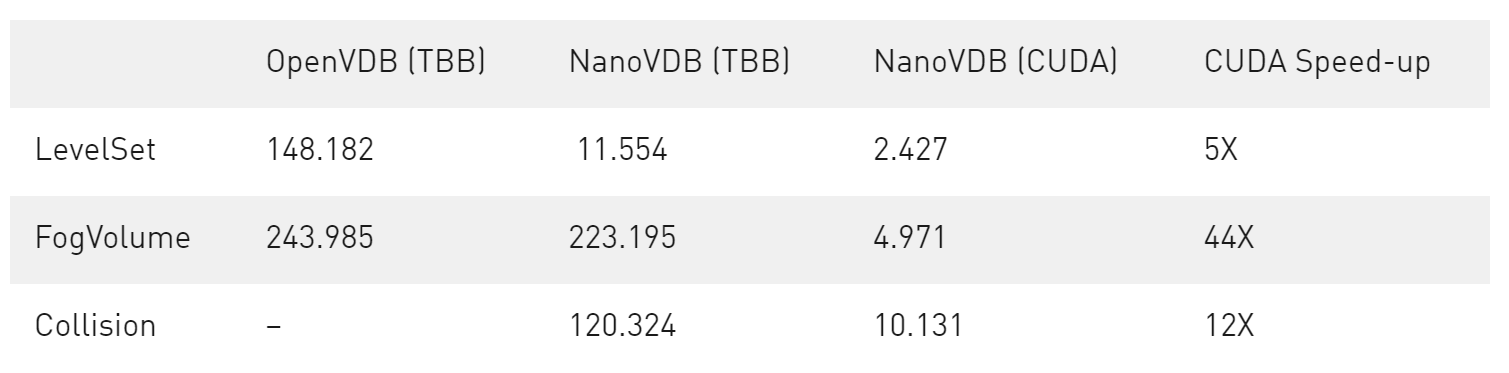
\includegraphics[width=0.75\textwidth]{res/nvidia_benchmark.png}
	\caption{Benchmark results published by NVIDIA. The benchmark setup and source code are undisclosed. \cite{nanovdb_nvidia}}
	\label{fig::nvidia_benchmark}
\end{figure}

For the process simulations the results for level-set raytracing are of significant importance. 
According to Fig. \ref{fig::nvidia_benchmark} NanoVDB on a GPU should be 60x faster compared to a multithreaded implementation using OpenVDB. (Execution time of 2.427ms vs 148.182ms).

However since the benchmark setup and source code are no published it is not clear if the same incerase in performance can be achieved for other applications.
Therefore the goal of this paper is to verify these results using a benchmark that is tailored to typical applications within the semiconductor process simulation.
\setcounter{section}{1}
\section{Methodology}

% Rendering images is usually achieved by casting a set amount of rays onto a 3D object and calculating all intersection points.
% Once an intersection is found a ray may spawn one or more rays at the intersection point in order to simulate effects such as reflections, glossy surfaces, semi-transparent materials, etc.
% It is also possible that no intersection is found if the ray leaves the bounding box. This is the equivalent of a ray "shooting into the sky".
% These rays do not contribute to the result and are usually discarded. 
% Since the exact point of exit is not required and no additional rays are spawned theses rays are cheaper to compute.


% \begin{figure}[H]
% 	\centering
% 	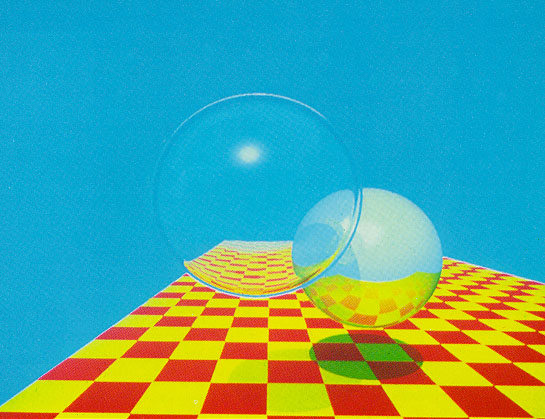
\includegraphics[width=0.5\textwidth]{res/rendered_image_turner.jpg}
% 	\caption{One of the first rendered digitally rendered images \cite{rendering_turner}. Approximately half of the rendered area represents the sky. Rays casted there can be discarded}
% 	\label{fig::rendered_image_turner}
% \end{figure}


% The main difference between image rendering and applications in Semiconductor Process Simulation is that there are usually no skyboxes.
% Furthermore it is undesirable to discard rays since they do not contribute to the simulation and are therefore wasted computing power.

The benchmark is designed to be baseline for future applications that are using NanoVDB for narrow-band level-sets and raytracing within the context of Semiconductor process simulation.
Therefore no specific problem is chosen but the worst-case scenario in a typical application is modelled. 


Source code, build instructions and measurement data are available at \footnote{Pre-Release version. The project is not finished yet}:
\\~\\
\centerline{\url{https://github.com/hitimr/SelectedTopicsCompElectronics}}


\subsection{Hardware setup}
The benchmark is performed on a single node of a scientific cluster provided by TU Wien. 
The node consists of the devices listed in Tab. \ref{tab:hardware} which are both used for the benchmark.

CPUs and GPUs are different platforms in terms of architecture and design which makes a fair comparison with regards to their technical aspects difficult.
However both devices are similar in cost of acquisition and operating expenses (i.e. power usage). 
Furthermore both platforms are marketed towards scientific computing.


\begin{table}[H]

\caption{Hardware used for the benchmark. Prices may fluctuate due to current events. Power consumption represents the absolute maximum ratings according to the vendor}
\centering
\begin{tabular}{@{}llll@{}}
	\toprule
	& Price           & Power Consumption & Cores                \\ \hline
Intel Xeon 6248 & € 3.300         & 105W              & 20 Cores; 40 Threads \\
NVIDIA Tesla T4 & € 2.500 - 3.000 & 70W               & 2.560 CUDA-Cores     \\ \bottomrule
\end{tabular}
\label{tab:hardware}
\end{table}


\subsection{Simulation environment}

A common problem in Semiconductor process simulation is light being cast into a trench with semi-reflective walls as shown in Fig. \ref{fig:benchmark_setup} (left).
To simplify the program and enforce a worst-case scenario the following modifications are performed:

\begin{itemize}
	\item Rays leaving the bounding box (i.e. shooting into the sky) are cheaper to compute but do not contribute to the simulation. 
	In order to prevent these edge cases rays are cast onto the inner surface of a hollow sphere.
	\item The point source is replaced with a volumetric source. Otherwise every ray would start within the same voxel which would lead to a beneficial memory access pattern.
	\item Depending on the reflecting angle, rays may cover different distances. Therefore the inner sphere (ray source) is offset to create a distribution of distances.
	\item Rays are shuffled in memory before being passed to the kernel to prevent beneficial memory access patterns.
	\item Any ray reflection on the surface is equivalent to having 2 separate rays (inbound and outbound) at the intersection point. Therefore reflections do not need to be modelled.
\end{itemize}


\begin{figure}[H]
	\centering
	% Rigth image
	\begin{subfigure}{0.35\textwidth}
	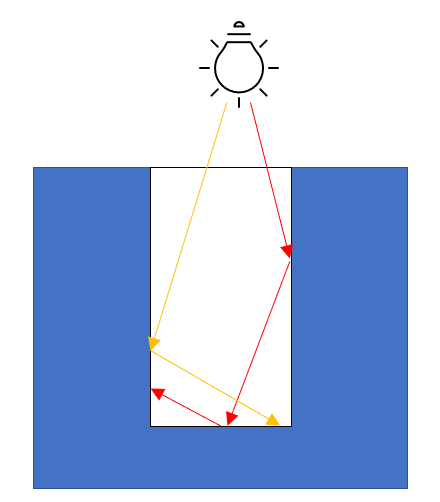
\includegraphics[width=1\linewidth]{res/trench_with_rays.png} 
	\caption{}
	%\label{fig:trench_with_rays}
	
\end{subfigure}
	% left image
	\begin{subfigure}{0.35\textwidth}
	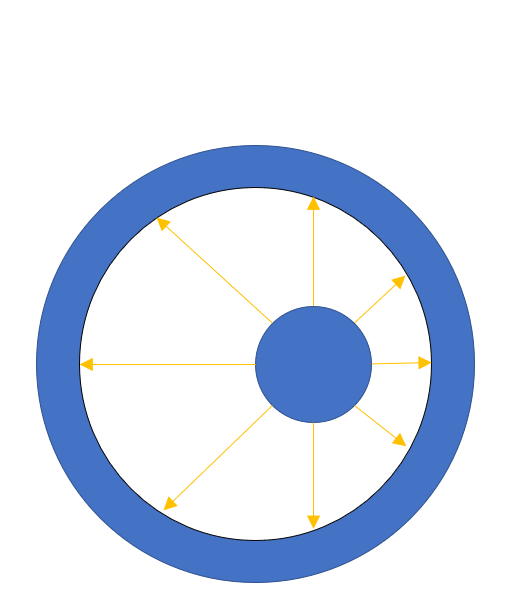
\includegraphics[width=1\linewidth]{res/benchmark_setup.png}
	\caption{}
	%\label{fig:parallel-solution}
\end{subfigure}

\caption{Benchmark setup. \textbf{a} Trench being illuminated by a light source. Every ray has a chance of being reflected or absorbed.
\textbf{b} 2D cross-section of the modified setup. For the benchmark rays are distributed evenly across the surface of the inner sphere.} 
\label{fig:benchmark_setup}
\end{figure}


Origin and direction of every ray along with a ground truth are precomputed and passed to three different ray intersection kernels:

\begin{itemize}
	\item OpenVDB (CPU)
	\item NanoVDB (CPU)
	\item NanoVDB (GPU)
\end{itemize}

The OpenVDB kernel servers as a baseline for comparison.
Both NanoVDB kernels are identical but launched on different platforms.

Only the time required to calculate intersections is measured. Memory management, data transfer, ray generation, result verification, etc. is not included.
After the benchmark is complete the number of calculated rays per second is derived using 

\begin{equation}
	Rps = \frac{ray \: count}{time} = [\frac{1}{s}]
\end{equation}

The benchmark is repeated while increasing the number of rays until no further increases in $Rps$ is observed. 
After each iteration the resulting intersections are compared to a pre-computed ground truth to assure the correctness of the results.
The asymptotic behaviour of the resulting performance curve is used to estimate a potential performance gain for switching to NanoVDB or GPUs.
%\include{2-conjugate-gradients}
%\section{Is this the real life?}



\begin{figure}[H]
	\centering
	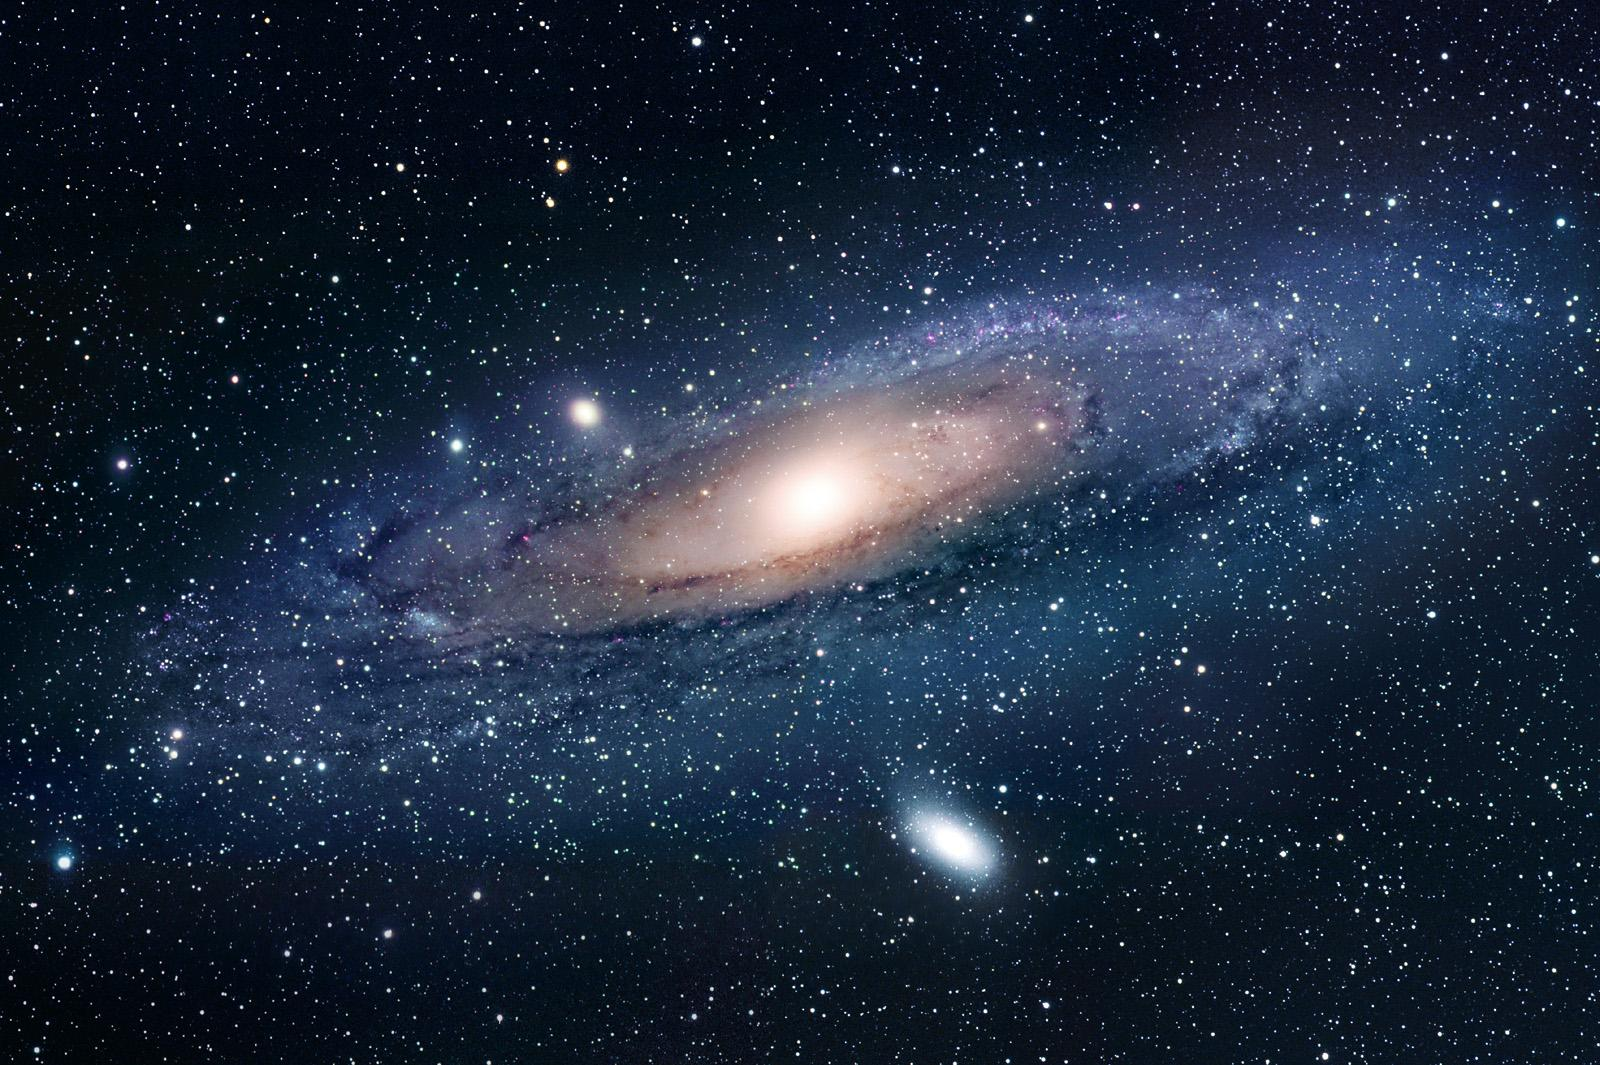
\includegraphics[width=0.75\textwidth]{res/sample-image.jpeg}
	\caption{A centered image}
	\label{fig::sample-label}
\end{figure}

\begin{figure}[h]
        % Rigth image
        \begin{subfigure}{0.45\textwidth}
        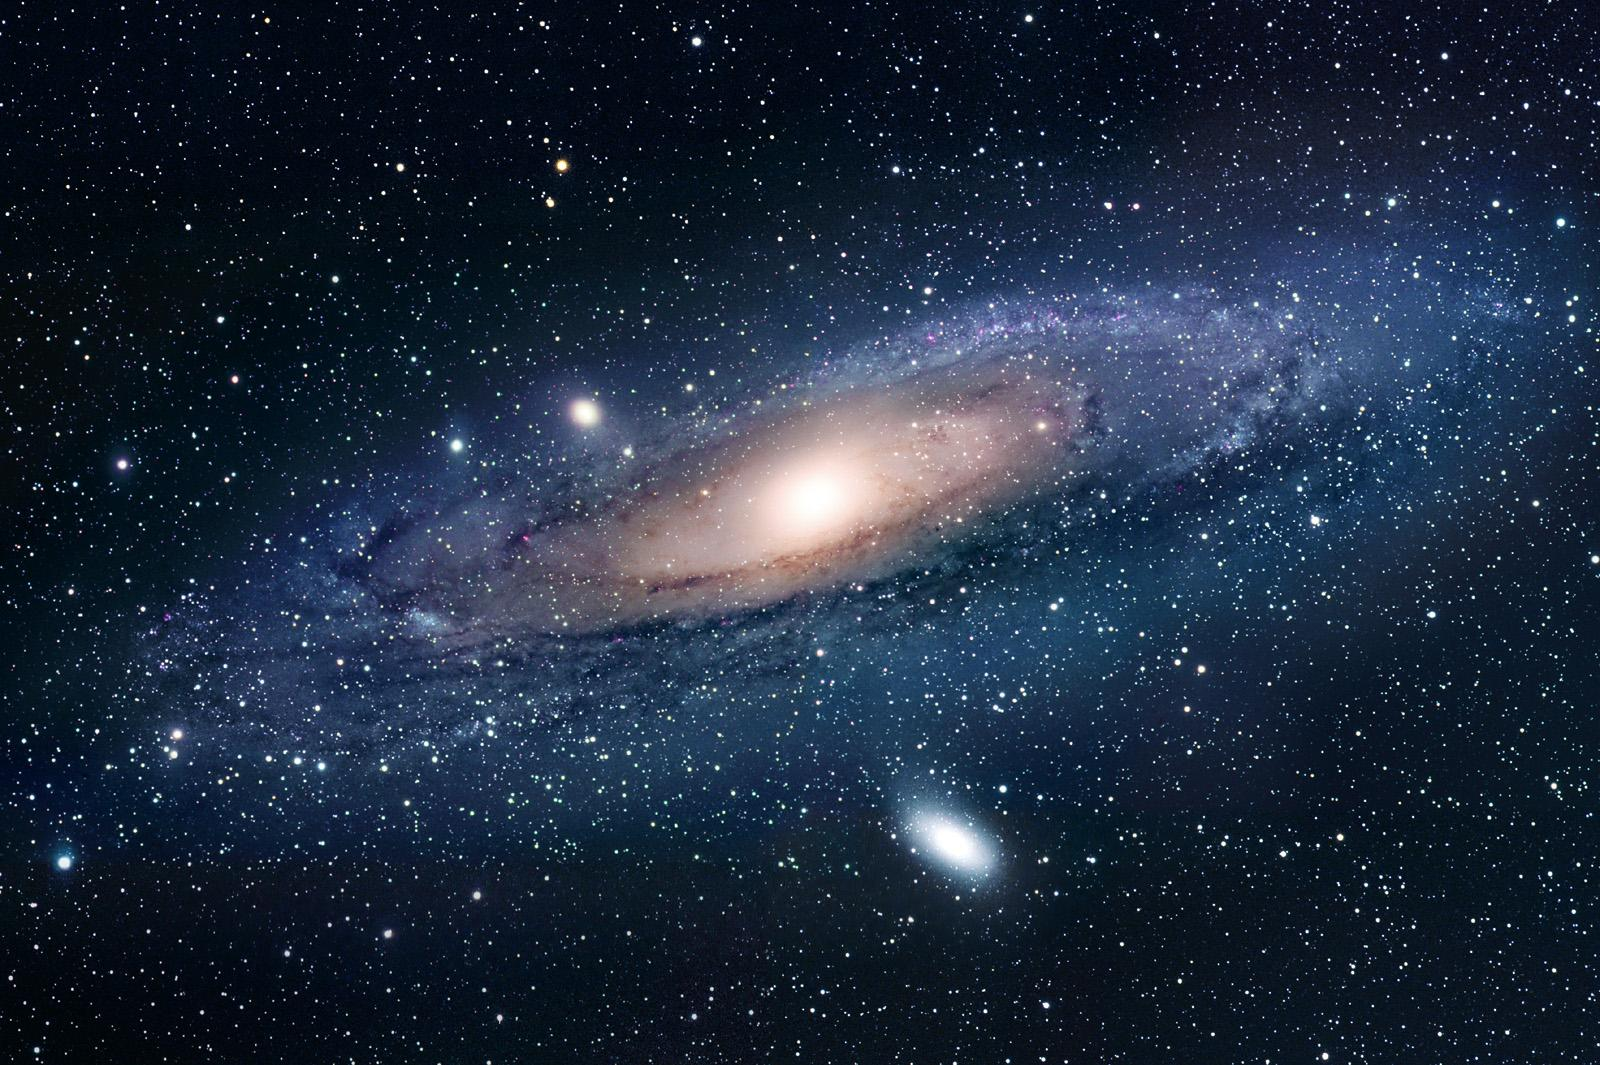
\includegraphics[width=1\linewidth]{res/sample-image.jpeg} 
        %\caption{Caption1}
        %\label{fig:serial-solution}
        
    \end{subfigure}
        % left image
        \begin{subfigure}{0.45\textwidth}
        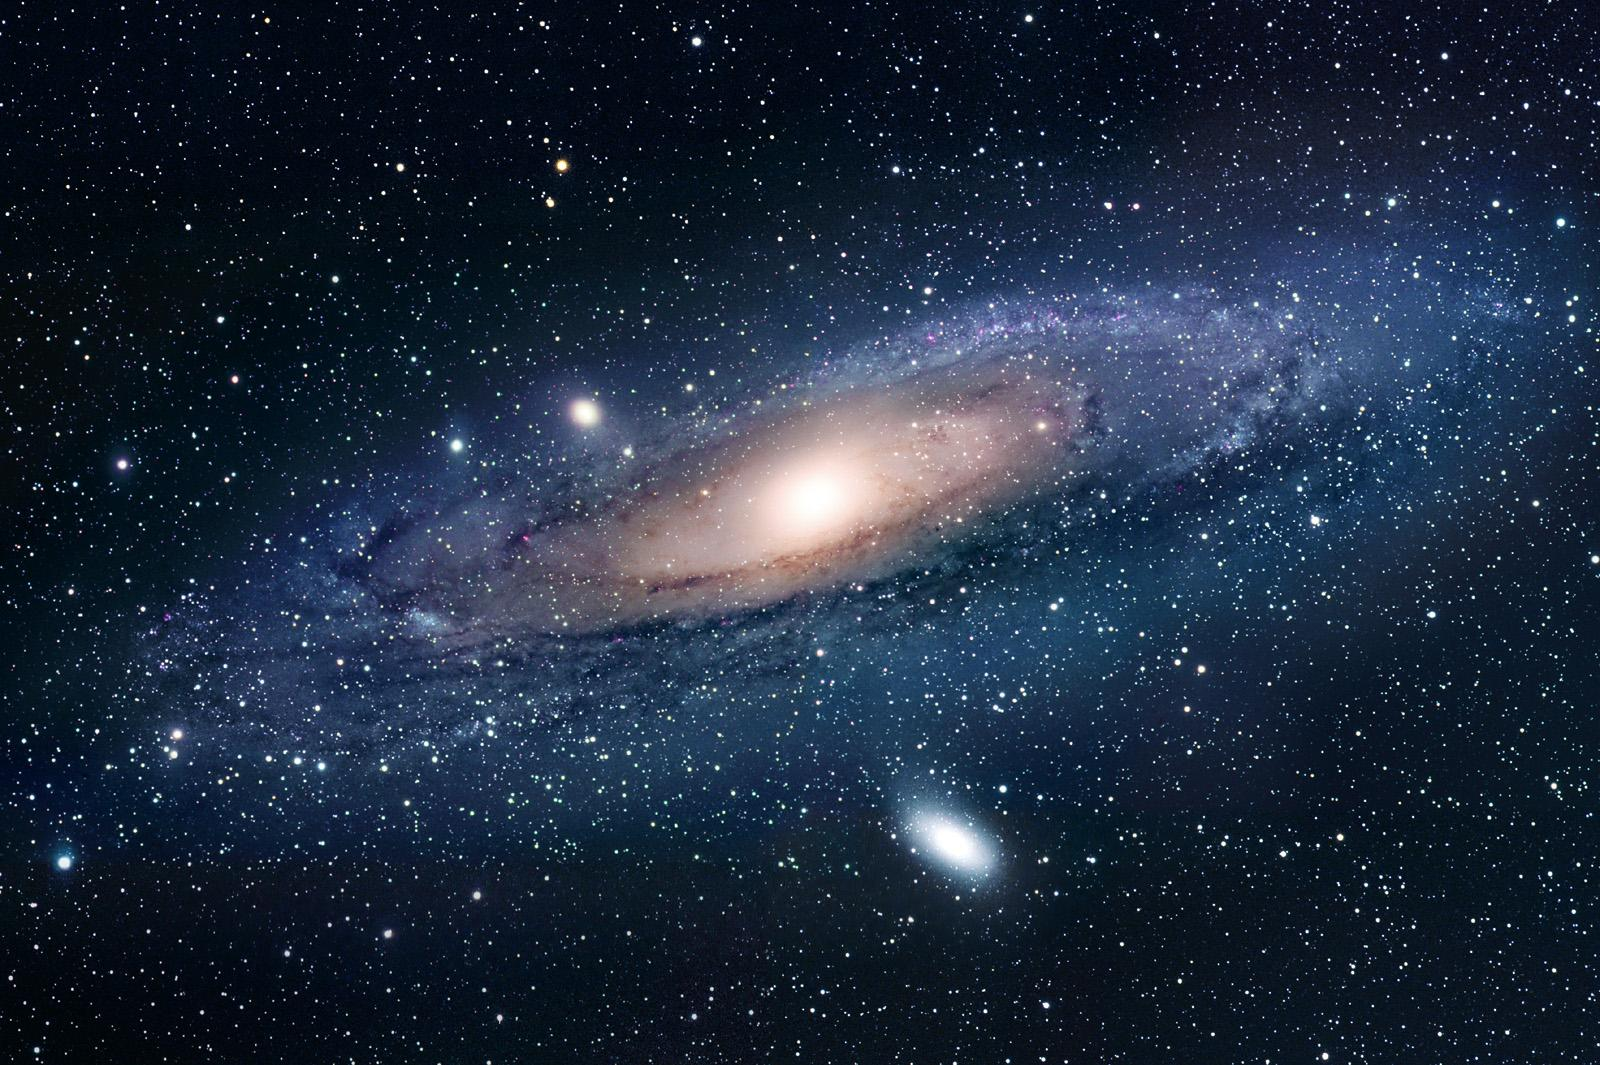
\includegraphics[width=1\linewidth]{res/sample-image.jpeg}
        %\caption{Caption 2}
        %\label{fig:parallel-solution}
    \end{subfigure}
    
    \caption{two images side-by-side}
    %\label{fig:serial-vs-parallel}
\end{figure}

\section{Is this just fantasy?}




%\begin{minipage}{\linewidth}
\begin{lstlisting}[caption={Sample Algorithm}]
int main()
{
    return 0;   // Comment
}
\end{lstlisting}
%\end{minipage}



\todo{remove sample chapter before release}


   
\printbibliography
\end{document}